\newpage
\section{Beschreiben der WS2812 LED Matrix aus dem Speicher (Aufgabe 8)}

\begin{figure}[H]
\centering
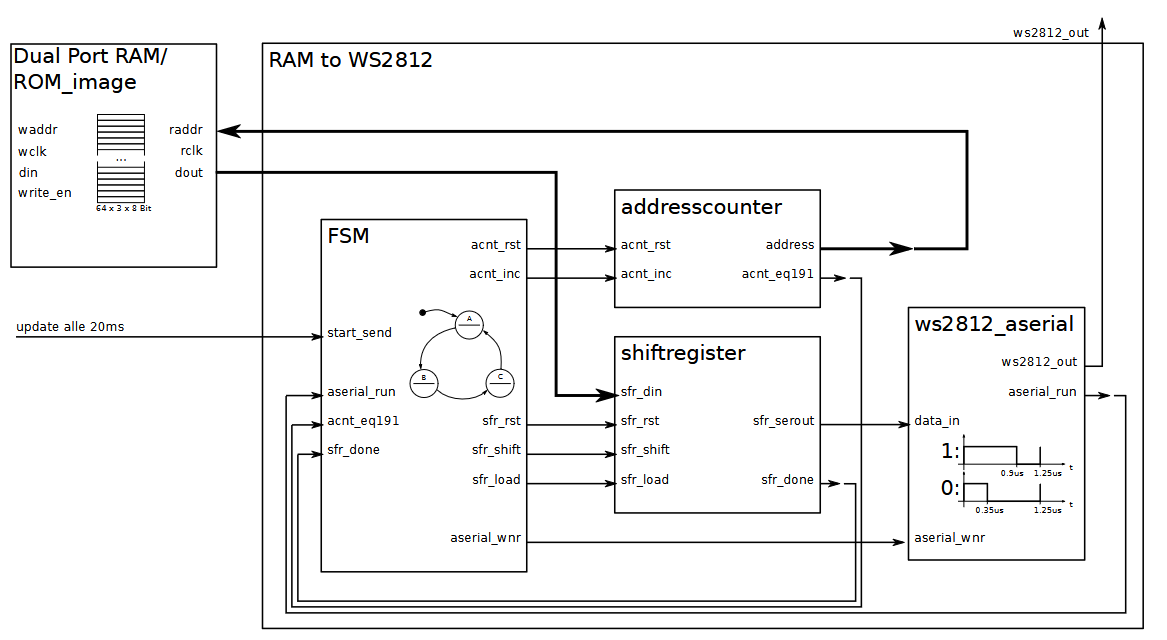
\includegraphics[width=\textwidth]{A8_Abgabe/res/blockschaltbild.png}
\caption{Blockschaltbild des RAMtoWS2812 Moduls}
\label{fig:blockschaltbild}
\end{figure}

Die Komponente \texttt{RAMtoWS2812} bildet die zentrale Schnittstelle zwischen dem Speicher und der seriellen Ansteuerung der 8×8-WS2812-Matrix. Wie in Abbildung~\ref{fig:blockschaltbild} dargestellt, liest die Schaltung die im Speicher abgelegten RGB-Daten sequentiell aus und serialisiert sie für die asynchrone Übertragung an die LED-Kette. Der Speicher ist als 8-Bit-RAM mit 192 Adressen organisiert -- je LED werden drei Byte für Grün, Rot und Blau benötigt, sodass insgesamt 64×3 = 192 Byte für die vollständige Matrixausgabe vorgehalten werden.


\subsection{Implementierung des WS2812-to-RAM Moduls}

Der Aufbau der Komponente gliedert sich in vier miteinander verknüpfte Module: Die \emph{addresscounter} erzeugt die sequentiellen Lesezugriffe auf den Speicher, das \emph{shiftregister} wandelt die parallelen 8-Bit-Werte in einen seriellen Bitstrom um, das \emph{ws2812\_aserial}-Modul erzeugt das zeitkritische WS2812-Protokoll für jedes einzelne Bit, und die \emph{FSM} koordiniert den zeitlichen Ablauf dieser drei Komponenten. Die FSM durchläuft dabei zyklisch die Zustände \texttt{IDLE}, \texttt{LOAD\_DATA} und \texttt{SENDING}, wobei im Zustand \texttt{LOAD\_DATA} jeweils ein neues Byte aus dem Speicher in das Schieberegister geladen und die Adresse inkrementiert wird, und im Zustand \texttt{SENDING} die acht Bits des aktuellen Bytes seriell übertragen werden.

\subsubsection{Finite-State-Machine}

\begin{figure}[H]
\centering
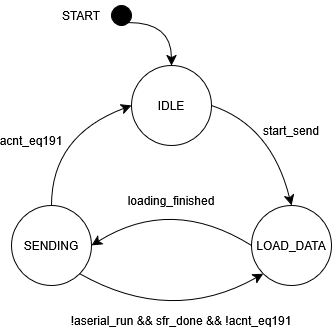
\includegraphics[width=0.5\textwidth]{A8_Abgabe/res/RAMtoWS2812_FSM.png}
\caption{Zustandsüberführungsdiagramm der FSM des WS2812-to-RAM Moduls}
\label{fig:WS2812toRAM_FSM}
\end{figure}

Die Zustandsmaschine startet im Zustand \texttt{IDLE} und wechselt bei aktivem \texttt{start\_send}-Signal nach \texttt{LOAD\_DATA}. Dort wird für die erste Adresse das Schieberegister geladen und das \texttt{aserial\_wnr}-Signal gesetzt, um die Übertragung des ersten Bits zu initiieren. Für alle folgenden Adressen wird zunächst der Adresszähler inkrementiert, bevor das neue Byte geladen wird. Nach Abschluss des Ladevorgangs wechselt die FSM in den Zustand \texttt{SENDING}. Hier wird das Schieberegister mit jedem Takt, in dem \texttt{aserial\_run} inaktiv ist, um eine Position weitergeschoben, wodurch das nächste Bit an den seriellen Ausgang gelangt. Sobald acht Verschiebeoperationen abgeschlossen sind, signalisiert \texttt{sfr\_done} der FSM, dass das Byte vollständig übertragen wurde. Die FSM kehrt dann nach \texttt{LOAD\_DATA} zurück, um das nächste Byte zu laden. Erreicht der Adresszähler den Wert 191, setzt \texttt{acnt\_eq191} die FSM zurück in den Zustand \texttt{IDLE}.

Dieser Entwurf der FSM wurde in dem folgenden Code implementiert:

\inputminted[linenos,frame=single,fontsize=\footnotesize]{vhdl}{A8_Abgabe/rtl/fsm.vhd}

\subsubsection{Addresscounter}

Der Adresszähler wird über \texttt{acnt\_rst} synchron auf Null zurückgesetzt und zählt bei jedem aktiv-high-Impuls auf \texttt{acnt\_inc} exakt um eins hoch. Die Inkrementierung erfolgt flankengesteuert: Ein internes Flipflop verhindert, dass ein dauerhaftes High-Signal zu mehrfachen Zählschritten führt. Sobald der Zählerstand 191 erreicht, wird \texttt{acnt\_eq191} aktiv und signalisiert der FSM das Ende des Bilddurchlaufs.

\inputminted[linenos,frame=single,fontsize=\footnotesize]{vhdl}{A8_Abgabe/rtl/addresscounter.vhd}

\subsubsection{Shiftregister}

Das Schieberegister dient als Puffer zwischen dem parallelen Speicherausgang und dem seriellen Protokollmodul. Mit \texttt{sfr\_load} wird der aktuelle 8-Bit-Wert von \texttt{sfr\_din} in das Register übernommen. Bei jedem aktiven \texttt{sfr\_shift} wird der Inhalt um eine Position nach links geschoben, wobei das höchstwertige Bit (MSB) am Ausgang \texttt{sfr\_serout} anliegt. Ein interner Zähler verfolgt die Anzahl der Verschiebeoperationen; nach sieben Schritten ist das niederwertigste Bit (LSB) am Ausgang angelegt, und \texttt{sfr\_done} wird aktiv.

\inputminted[linenos,frame=single,fontsize=\footnotesize]{vhdl}{A8_Abgabe/rtl/shiftregister.vhd}

\subsubsection{WS2812-to-RAM Hauptmodul}

Die Hauptkomponente \texttt{RAMtoWS2812} integriert die drei Submodule und steuert den Datenfluss entsprechend der FSM-Logik. Sie empfängt die 8-Bit-Daten vom RAM, lädt sie in das Schieberegister, und koordiniert die serielle Ausgabe über das WS2812-Protokoll. Das Modul ist so konzipiert, dass es kontinuierlich die 192 Adressen des Speichers durchläuft und die entsprechenden RGB-Werte an die LED-Matrix sendet, bis der gesamte Bildzyklus abgeschlossen ist.

Ein wesentlicher Aspekt der Protokollsteuerung ist das Handshaking zwischen FSM, Schieberegister und seriellem Ausgangsmodul. Das Signal \texttt{aserial\_wnr} bleibt während der gesamten Übertragung eines Bytes aktiv und wird erst nach dem letzten Bit deaktiviert, um den abschließenden Reset-Code der WS2812-Kette zu ermöglichen. Das Signal \texttt{aserial\_run} zeigt an, dass ein Bit aktiv versendet wird; es wird jedoch zwischen zwei Bits mindestens für einen Taktzyklus inaktiv, was der FSM das Setzen des nächsten Bits am \texttt{data\_in}-Eingang ermöglicht, ohne dass zeitliche Überlappungen auftreten. Diese kurze Pause ist ausreichend, da das WS2812-Protokoll die Datenleitung bis zum Zeitpunkt 350~ns auf High hält -- unabhängig davon, ob eine \texttt{1} oder \texttt{0} gesendet wird.

\inputminted[linenos,frame=single,fontsize=\footnotesize]{vhdl}{A8_Abgabe/rtl/RAMtoWS2812.vhd}

\subsection{Simulation des WS2812-to-RAM Moduls}

Um die Funktionalität des \texttt{RAMtoWS2812}-Moduls zu überprüfen, wurde eine Testbench erstellt, die den RAM durch einen ROM mit vordefinierten RGB-Werten ersetzt und die Ausgabe an die WS2812-Kette simuliert. In der Testbench wird 

\inputminted[linenos,frame=single,fontsize=\footnotesize]{vhdl}{A8_Abgabe/sim/RAMtoWS2812_tb.vhd}

% Platzhalter für die Simulationsergebnisse, die gleich noch eingefügt werden.

\subsection{Synthese und Test des WS2812-to-RAM Moduls}

Für den ersten Funktionstest wurde das Dual-Port-RAM durch ein ROM aus dem Package \texttt{const\_image} ersetzt. Das ROM enthält vordefinierte Bildmuster als konstante Arrays vom Typ \texttt{grb\_bmp\_t} mit 192 Einträgen zu je 8 Bit. Die Adressierung erfolgt direkt über den Ausgang des Adresszählers, wobei die Daten mit einem Takt Verzögerung am Ausgang \texttt{dout} bereitstehen. Diese Vereinfachung erlaubt es, die korrekte Funktionsweise der seriellen Ansteuerung zu verifizieren, zunächst ohne die Komplexität eines schreibbaren RAMs.

\inputminted[linenos,frame=single,fontsize=\footnotesize,firstline=0,lastline=15]{vhdl}{A8_Abgabe/rtl/romimages.vhd}

Diese ROM-Images wurden in einer separaten Entität definiert, um die Übersicht zu wahren und die Wiederverwendbarkeit zu erhöhen.

\inputminted[linenos,frame=single,fontsize=\footnotesize]{vhdl}{A8_Abgabe/rtl/rom.vhd}


Nach erfolgreicher Simulation wurde das Design synthetisiert und auf dem Iceduino-Board getestet. Der Ausgang \texttt{ws2812\_out} wurde dabei auf Pin~3 des PMOD3-Headers gelegt, der mit FPGA-Pin~8 verbunden ist. Die WS2812-Matrix wurde mit 5~V und GND über die Arduino-Header versorgt. Die Darstellung der vordefinierten ROM-Bilder bestätigte die korrekte Umsetzung des seriellen Protokolls und die zeitgerechte Ansteuerung aller 64 LEDs.

\begin{figure}[H]
\centering
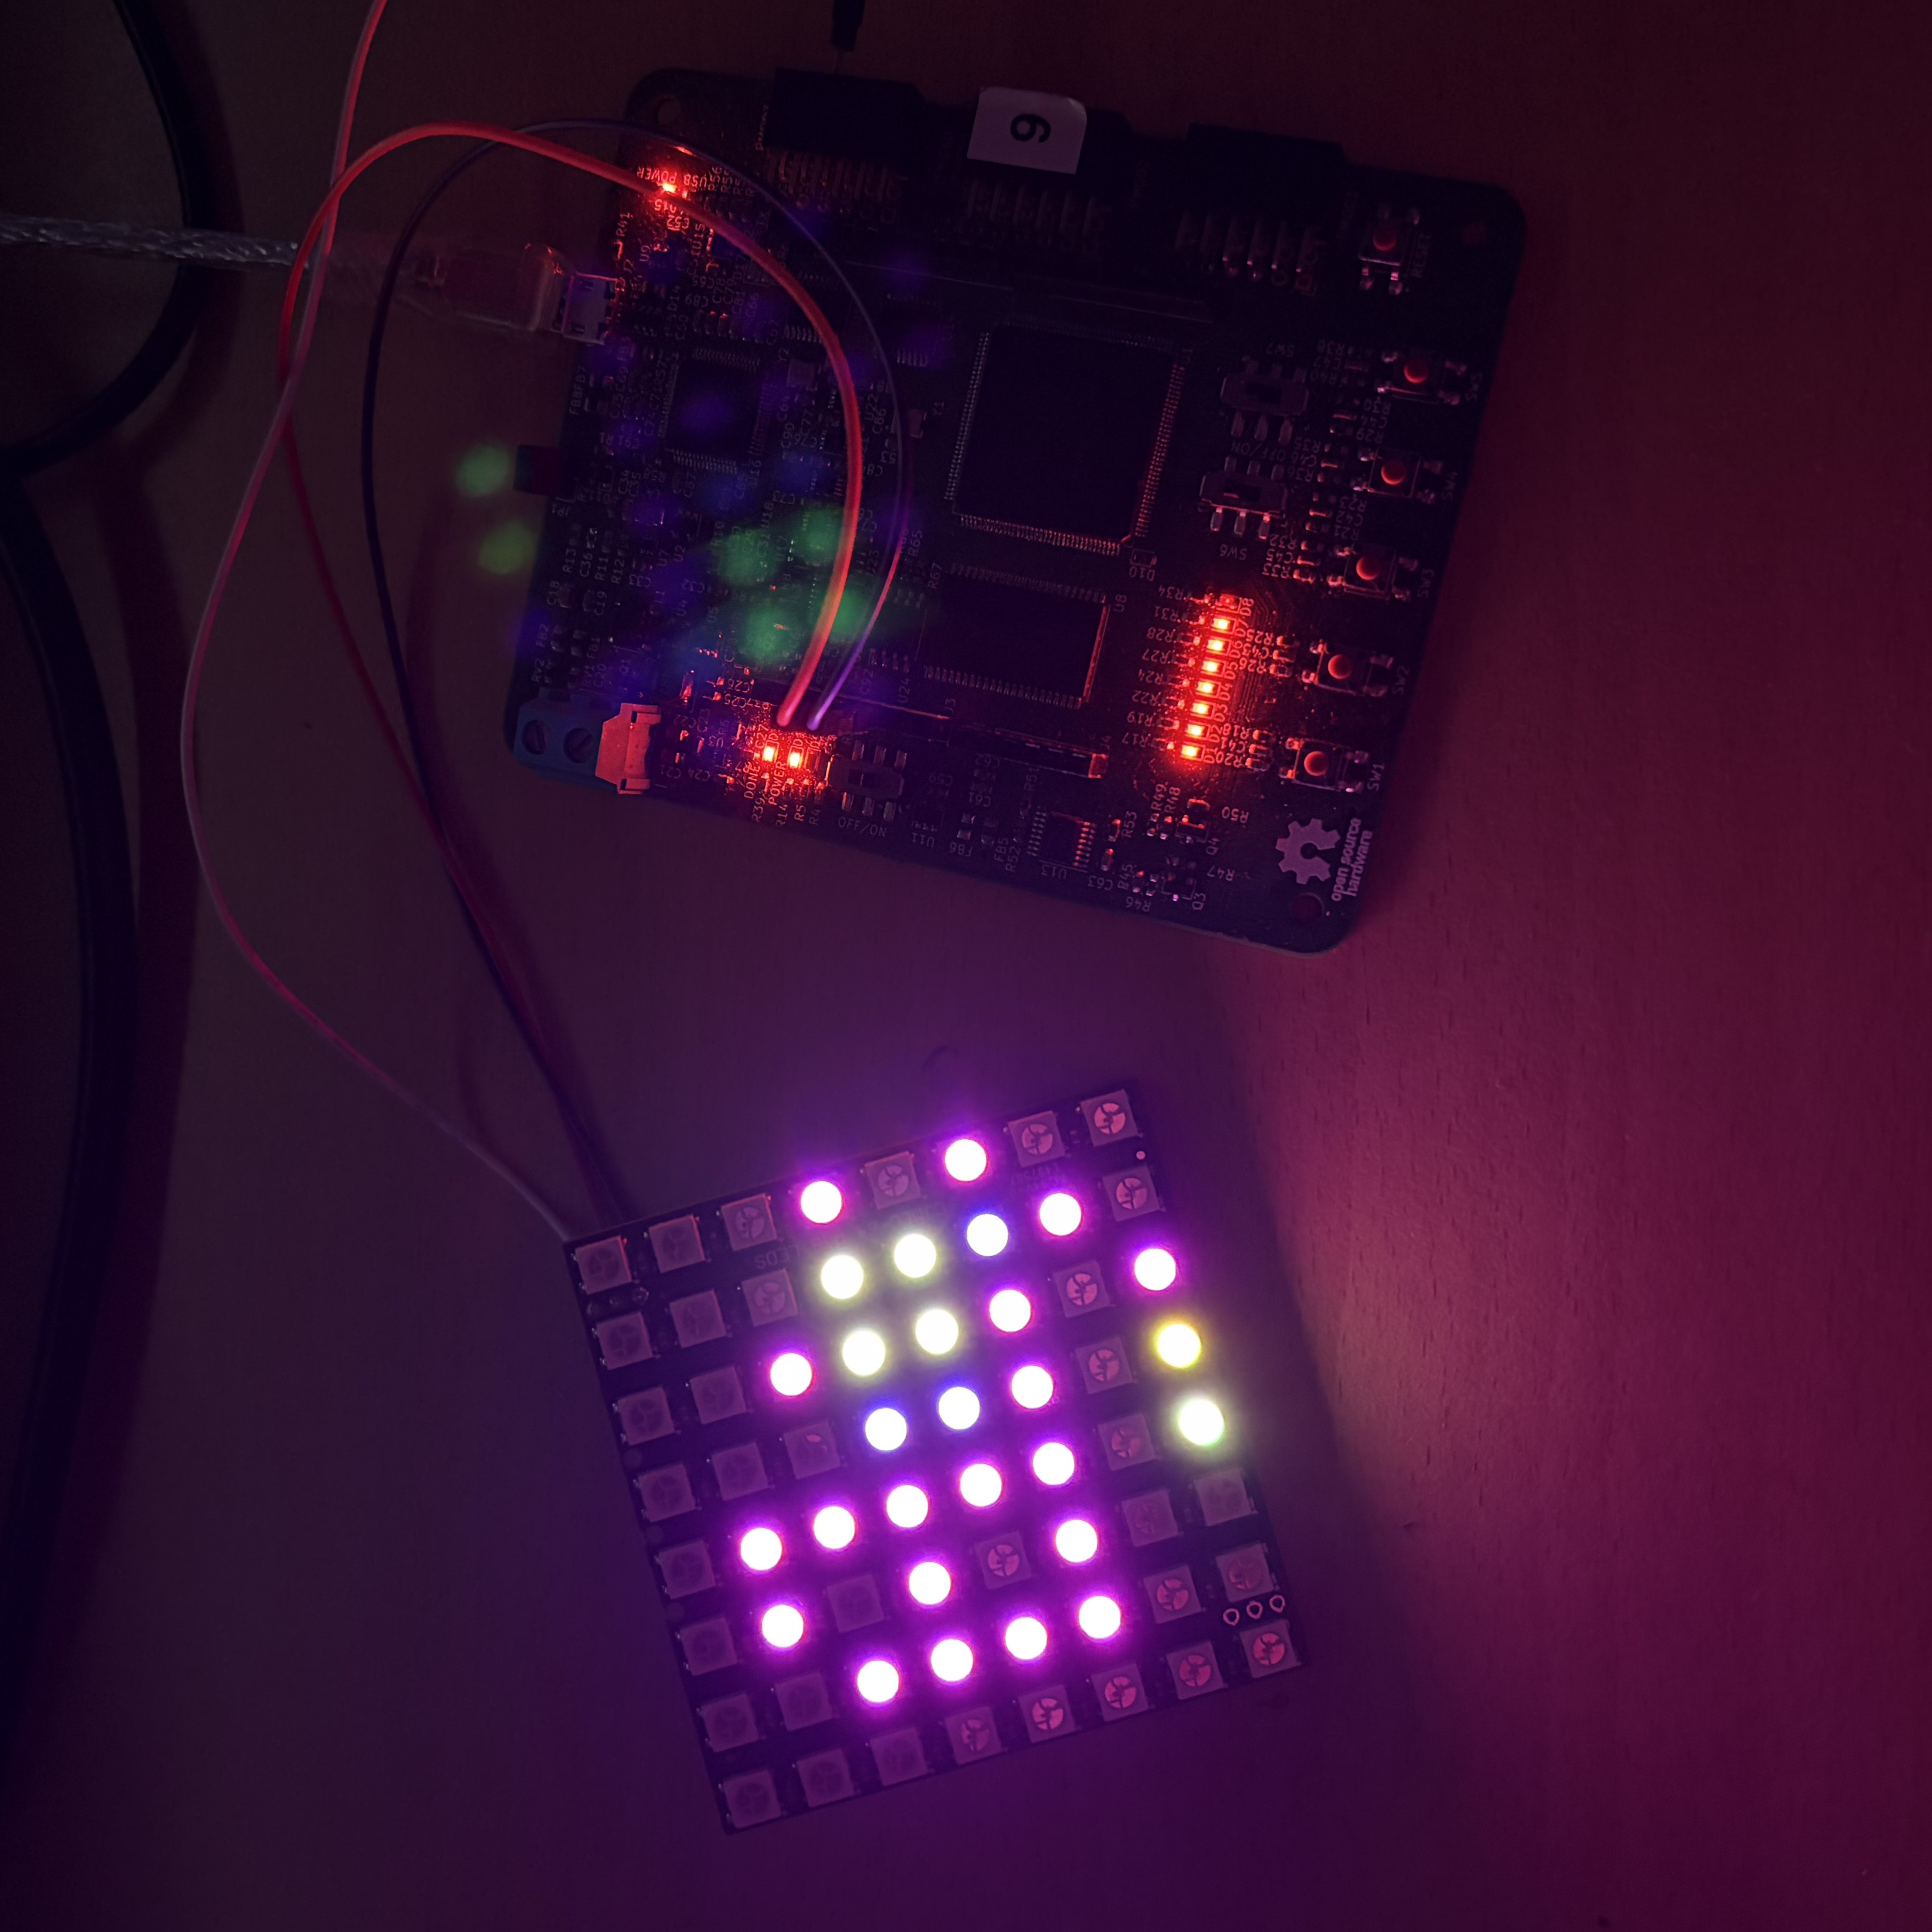
\includegraphics[width=\textwidth,angle=180]{A8_Abgabe/res/RAMtoWS2812_test1.jpeg}
\caption{Darstellung des ersten ROM Images auf der WS2812 LED Matrix}
\label{fig:RAMtoWS2812_test1}
\end{figure}

\begin{figure}[H]
\centering
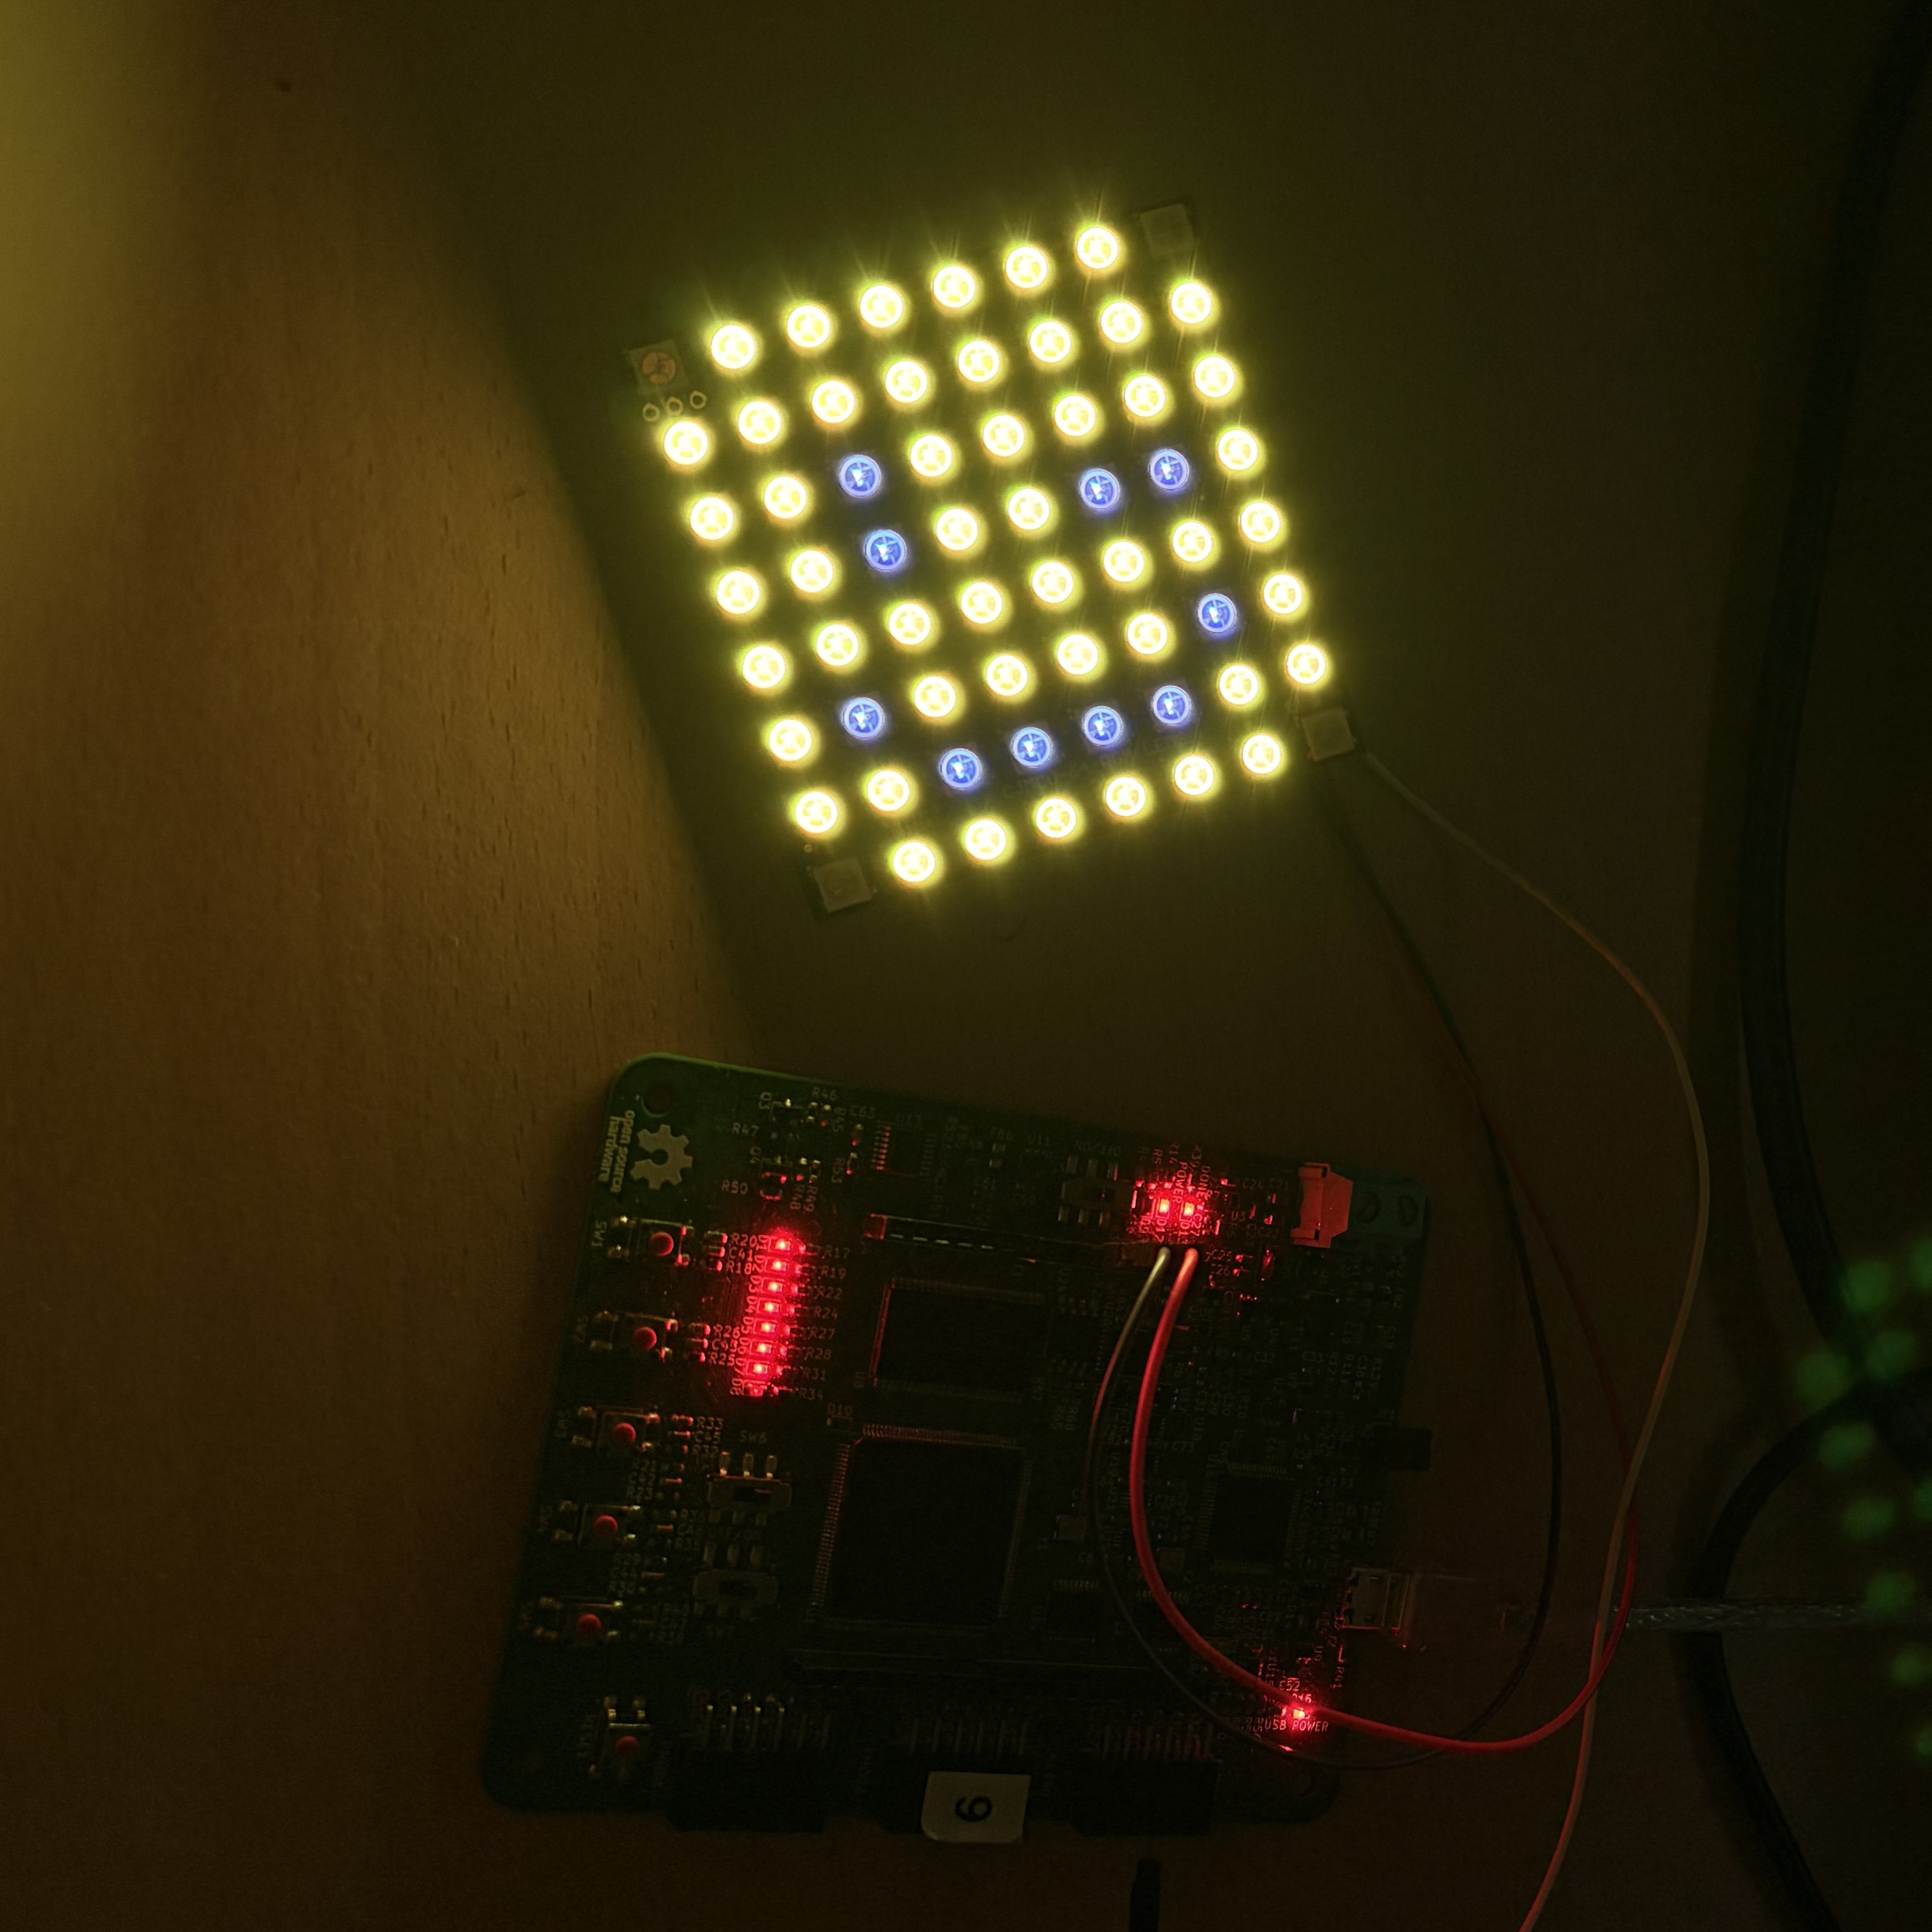
\includegraphics[width=\textwidth]{A8_Abgabe/res/RAMtoWS2812_test2.jpeg}
\caption{Darstellung des zweiten ROM Images auf der WS2812 LED Matrix}
\label{fig:RAMtoWS2812_test2}
\end{figure}

Es ist zu erkennen, dass die Bilder korrekt auf der LED-Matrix dargestellt werden. Das erste Bild zeigt ein einen kleinen Dinosaurier, das zweite Bild stellt ein Smiley-Gesicht dar. Diese Ergebnisse bestätigen die erfolgreiche Implementierung und Funktionalität des \texttt{RAMtoWS2812}-Moduls.
